\documentclass[11pt]{article}
\usepackage{graphicx}
\usepackage{geometry}
\usepackage{amsmath}
\usepackage{hyperref}
\usepackage{caption}      % 让图注更紧凑
\usepackage{subcaption}   % 若需要子图题

\geometry{a4paper, margin=0.95in}   % 页边距略缩小

\title{Project 3 Phase 1: State Estimation using Extended Kalman Filter}
\author{SIT IOK LONG, SID: 21100786}
\date{\today}

\begin{document}

\maketitle

\section{Methodology}
\vspace{-5pt}
\textbf{State and Prediction.}
The filter estimates the 15‑dimensional state
$\mathbf{x}=[\mathbf{p},\boldsymbol{\theta},\mathbf{v},\mathbf{b}_g,\mathbf{b}_a]^\top$
(position, Euler angles, velocity, gyro/accel biases). The continuous dynamics use bias‑compensated IMU readings $\boldsymbol{\omega}=\boldsymbol{\omega}_m-\mathbf{b}_g$, $\mathbf{a}=\mathbf{a}_m-\mathbf{b}_a$:
\[
\dot{\mathbf{p}}=\mathbf{v},\qquad \dot{\boldsymbol{\theta}}=\boldsymbol{\omega},\qquad
\dot{\mathbf{v}}=\mathbf{R}(\boldsymbol{\theta})\mathbf{a}+\mathbf{g},
\]
with $\mathbf{g}=(0,0,-9.81)$ and bias random walks $\dot{\mathbf{b}}_g=\mathbf{n}_{bg}$, $\dot{\mathbf{b}}_a=\mathbf{n}_{ba}$.

Discrete prediction uses forward Euler for the mean, and a first‑order covariance propagation:
\[
\mathbf{x}_{k+1}^- = \mathbf{f}(\mathbf{x}_k,\boldsymbol{\omega}_k,\mathbf{a}_k,dt),\qquad
\mathbf{P}_{k+1}^- = \mathbf{F}_d \mathbf{P}_k \mathbf{F}_d^\top + \mathbf{U}\mathbf{Q}\mathbf{U}^\top dt,
\]
with $\mathbf{F}_d=\mathbf{I}+\mathbf{F}dt$ and $\mathbf{Q}$ diagonal containing IMU noise densities.

\textbf{Visual Measurement.}
The tag detector provides the camera pose in the world frame. Using the extrinsic calibration (camera‑to‑IMU translation $(0.05,0.05,0)$~m, rotation $\mathbf{R}_c^i=\mathrm{diag}(1,-1,-1)$), we convert it to the IMU frame:
\[
\mathbf{p}_{\mathrm{IMU}}^w = \mathbf{p}_{\mathrm{cam}}^w - \mathbf{R}_{\mathrm{cam}}^w\,\mathbf{p}_{\mathrm{cam}}^{\mathrm{IMU}},\qquad
\mathbf{R}_{\mathrm{IMU}}^w = \mathbf{R}_{\mathrm{cam}}^w (\mathbf{R}_c^i)^\top.
\]
The measurement residual $\mathbf{y}=\mathbf{z}-\mathbf{H}\hat{\mathbf{x}}^-$ (position and Euler angles) is computed; yaw is wrapped to $[-\pi,\pi)$.

\textbf{Mahalanobis Gating.}
To reject outliers, we check the squared Mahalanobis distance
$D^2 = \mathbf{y}^\top \mathbf{S}^{-1}\mathbf{y}$ with $\mathbf{S}=\mathbf{H}\mathbf{P}^-\mathbf{H}^\top+\mathbf{R}_t$.
If $D^2 > 16.81$ (99\% $\chi^2(6)$), the measurement is discarded. Otherwise, the standard EKF update is applied:
$\mathbf{K}=\mathbf{P}^-\mathbf{H}^\top\mathbf{S}^{-1}$, $\mathbf{x}^+=\mathbf{x}^-+\mathbf{K}\mathbf{y}$, $\mathbf{P}^+=(\mathbf{I}-\mathbf{K}\mathbf{H})\mathbf{P}^-$.

\newpage
\section{Results}

\begin{figure}[h]
    \centering
    \begin{minipage}{0.48\textwidth}
        \centering
        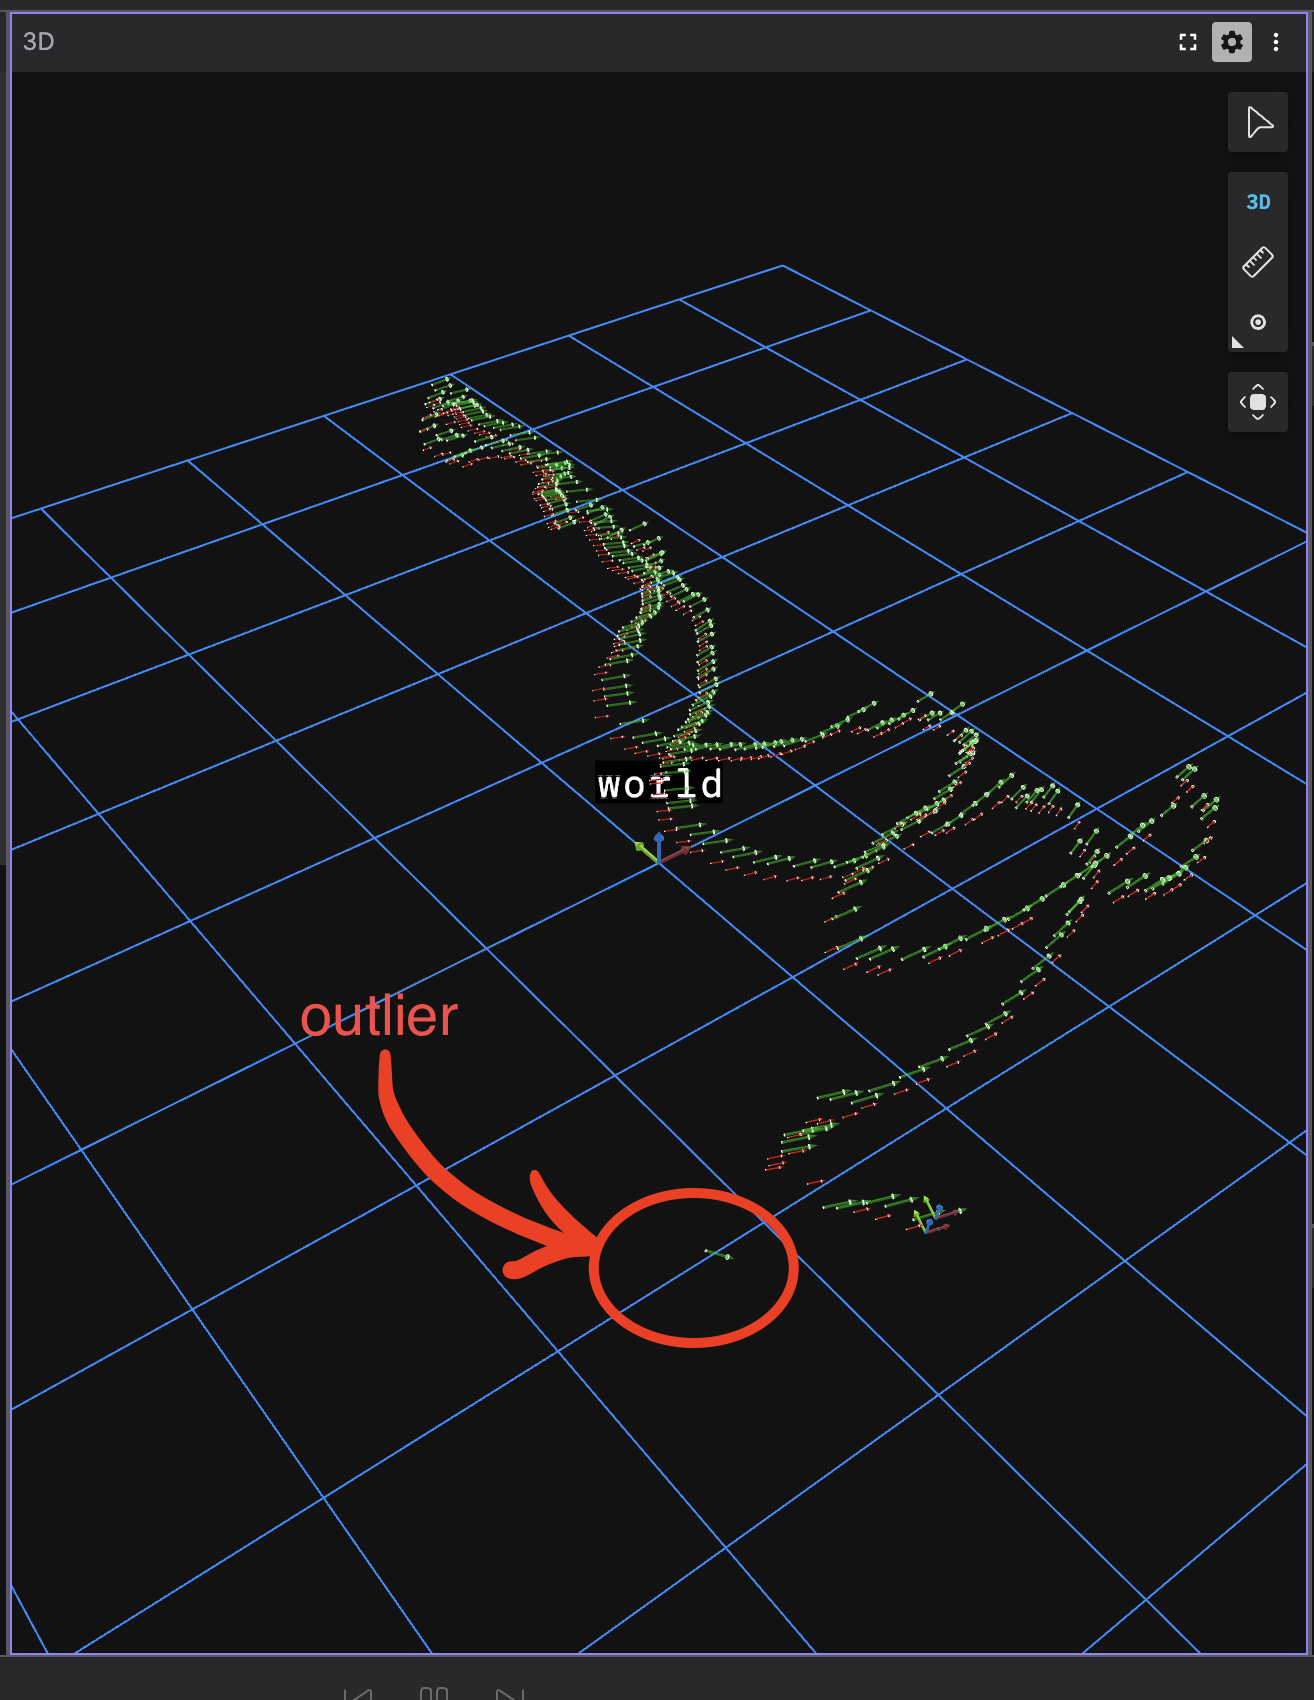
\includegraphics[width=\textwidth]{image1.png}
        \captionof{figure}{Trajectory in Foxglove: red arrow = EKF odom (\texttt{/ekf/ekf\_odom}), green arrow = raw tag detection (\texttt{/tag\_detector/odom\_ref}).}
        \label{fig:foxglove}
    \end{minipage}
    \hfill
    \begin{minipage}{0.48\textwidth}
        \centering
        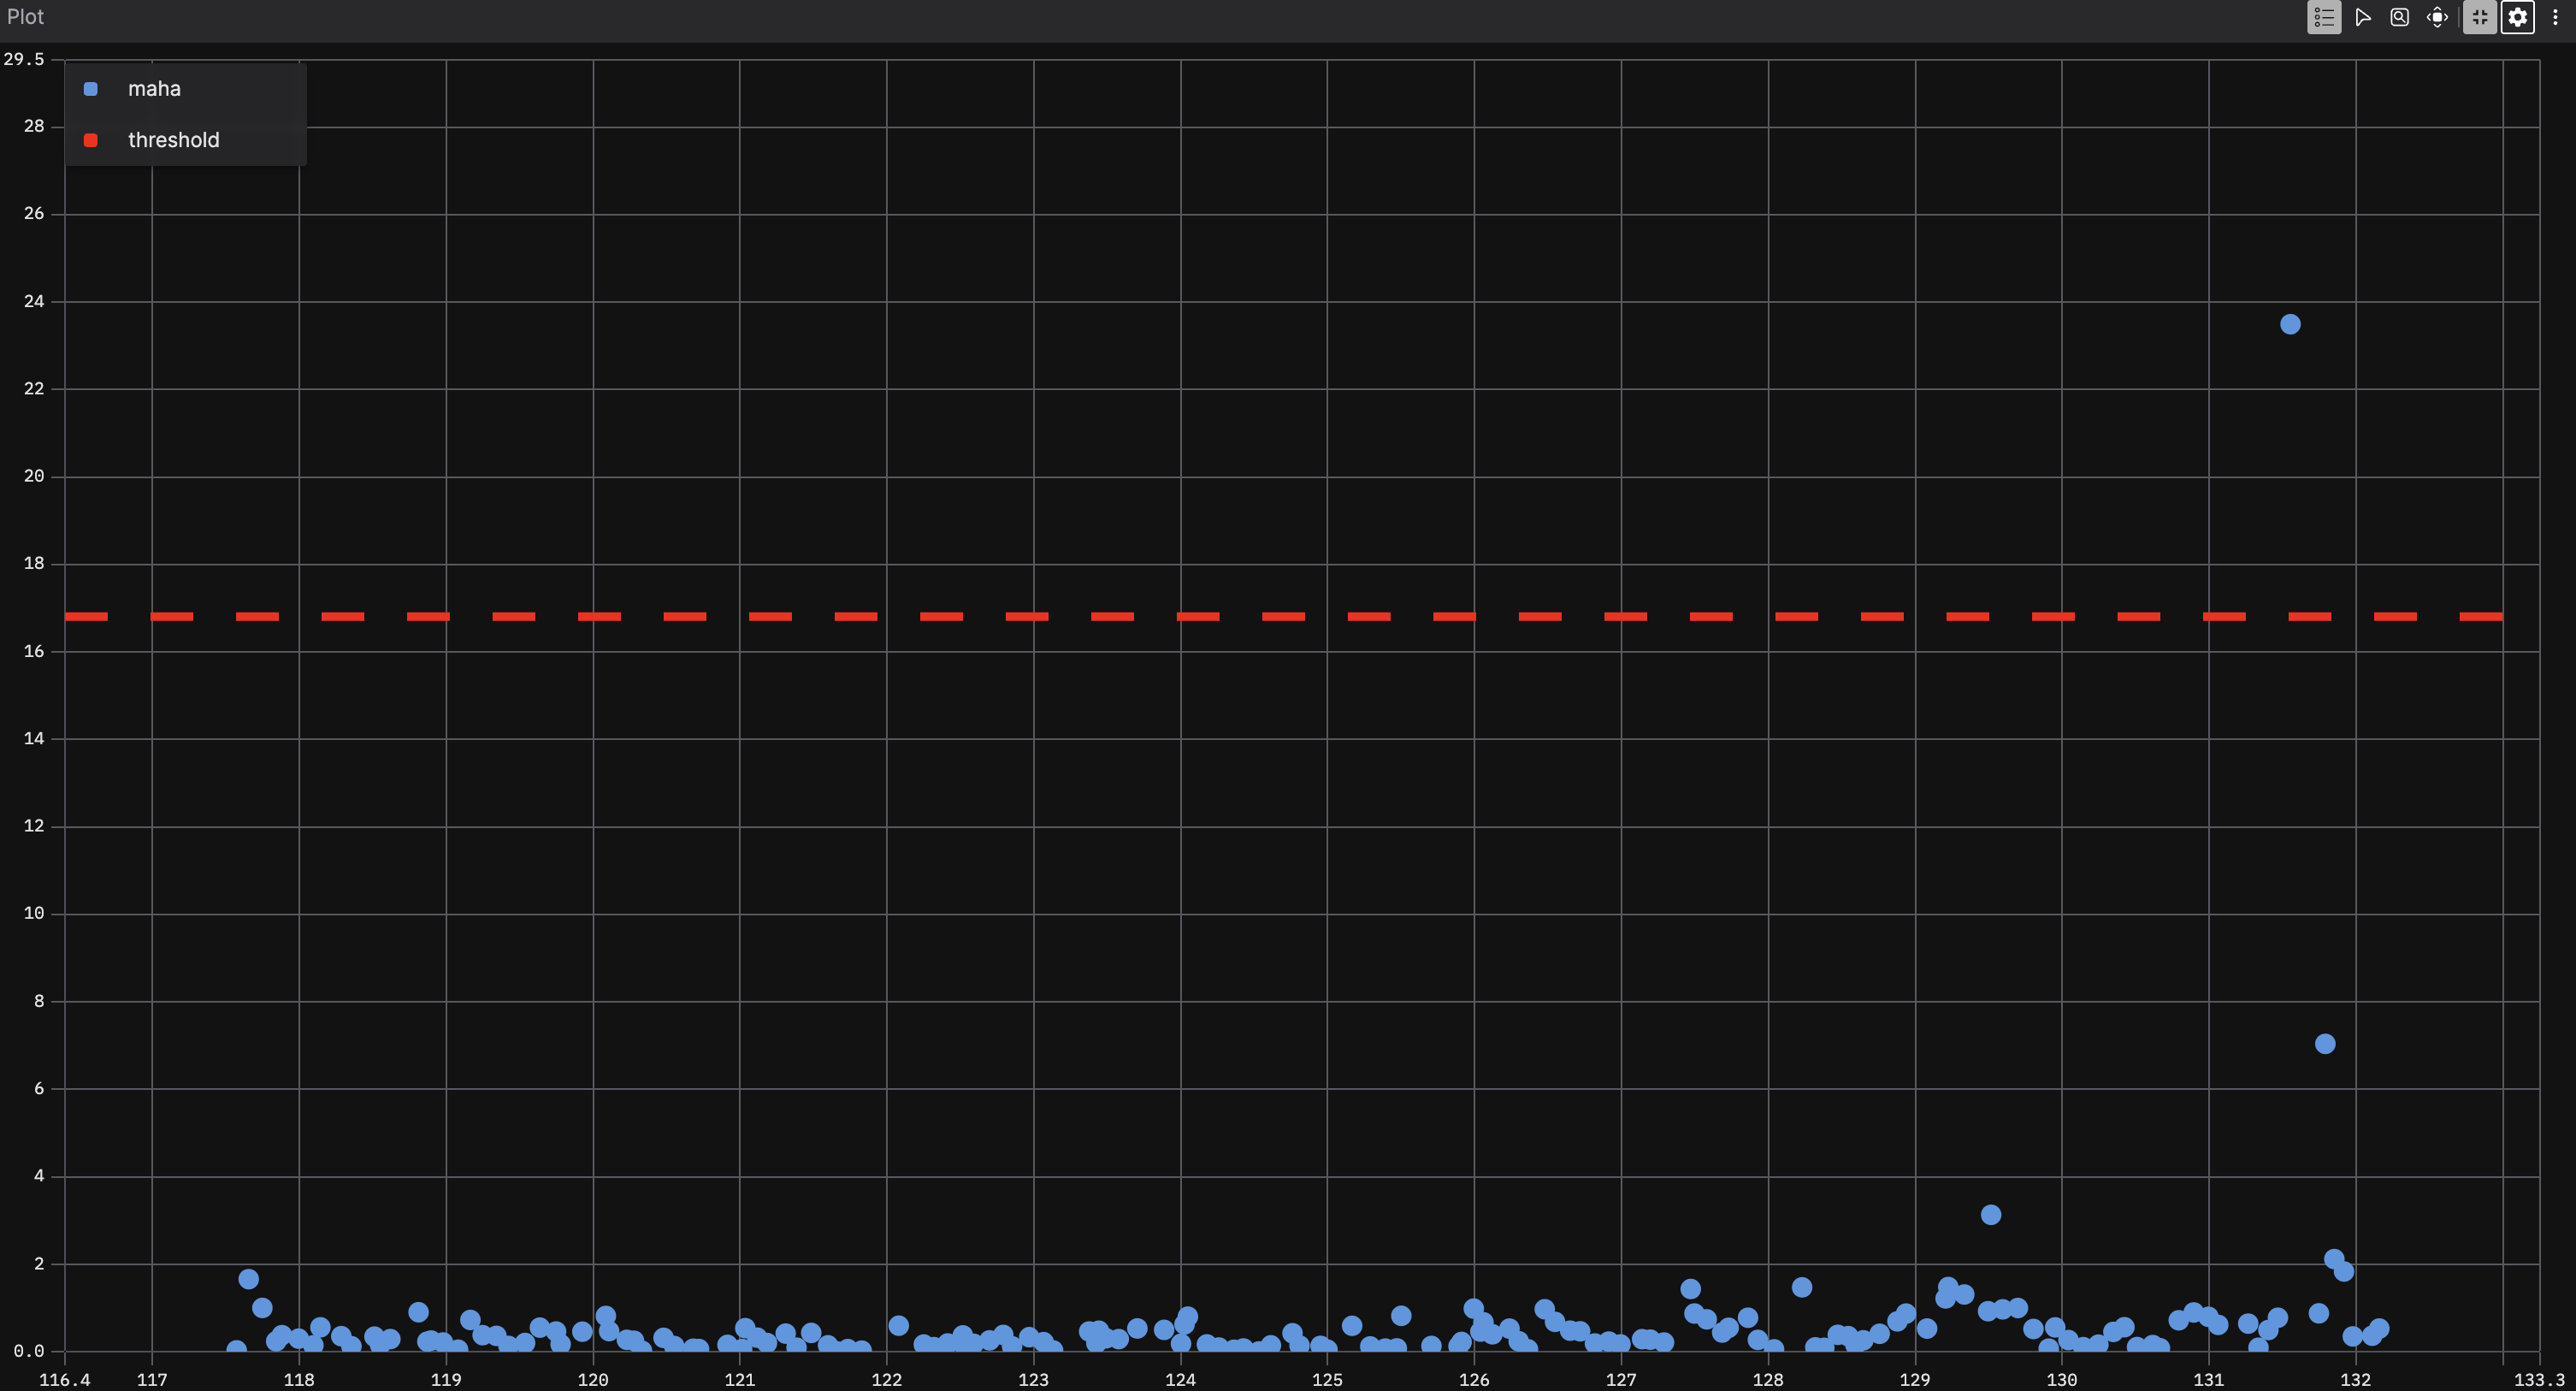
\includegraphics[width=\textwidth]{image2.png}
        \captionof{figure}{Mahalanobis gating: The outlier (red dashed threshold 16.81) triggers rejection, preventing a large state jump.}
        \label{fig:gating}
    \end{minipage}
\end{figure}

\section{Analysis and Tuning}
\vspace{-3pt}
\textbf{P/Rt Ratio.} The logged ratios $\mathbf{P}_{ii}/\mathbf{R}_{t,ii}$ for position and attitude remained consistently in the 0.5--1.0 band, confirming a balanced filter where prediction and measurement are trusted similarly.

\textbf{Parameters.} The measurement noise was set to
$\operatorname{diag}(0.002,0.002,0.025,0.004,0.004,0.025)$,
giving horizontal $\sim\!1.4$~cm, vertical $\sim\!5$~cm, and attitude $\sim\!2.3^\circ$--$4.5^\circ$ standard deviations. Process noise spectra in $\mathbf{Q}$ were increased to handle quick manoeuvres: gyro $2\,\mathrm{rad/s/\sqrt{Hz}}$, accel $5\,\mathrm{m/s^2/\sqrt{Hz}}$, gyro bias walk $5\times10^{-3}$, accel bias walk $5\times10^{-2}$. This kept innovations white and $D^2$ mostly within the expected $\chi^2$ bounds while gating out occasional visual outliers.

\textbf{Stability.} The filter ran stably over the entire rosbag without divergence. The Euler‑angle parametrisation is a potential limitation (gimbal lock at $\pm90^\circ$ pitch), but the test trajectory never approached those angles. A quaternion‑based error‑state EKF would be a straightforward extension for more aggressive motions.

\begin{thebibliography}{1}
\vspace{-5pt}
\bibitem{lect8} ELEC 5660 Lecture Notes, L8 -- Extended Kalman Filter.
\end{thebibliography}

\end{document}